\chapter{Development of full-stack microscopy}
\section{Observing with an instrument}
\paragraph*{} The scientific process to describe reality starts with making an observation. However, since reality seems too complex to be observed all at once, an approach evolved to study the universe in parts, with the human choosing the parts more essential than others to form a picture of the entirity. The picture is painted with the help of math, science and technology, that allows for the details of reality to be captured in numbers. The numbers are interpreted to arrive at conclusions on specific questions about the reality.

\paragraph*{} The process of acquiring information of reality in biology at the micron (10E-6 meter) scale involves the use of a microscope. A microscope is effective at observing entities that are unobservable by naked eye. 

\paragraph*{}The instrument is used to make repeated observations to record a phenomenon. The discovery of a phenomenon, and attributing it to structural biology, or genetics, has been the primary areas of thrust of recent biology.




\section{Limitations in microscopy software}
\subsection{Overview of existing technology}
\subsection{Requirements of community}
\subsection{Opportunities in open source development}
\section{Solution}
\subsection{Software architecture}
\subsection{Advantages}
\subsection{}

\paragraph*{} Existing microscope software requires a human operator to scan the sample visually, and identify regions of interest for imaging sample objects. However, it is difficult for the human user to manually comb through the sample to find fields of interest. Combing the sample for objects can also expose it to large amount of light, which can cause photobleaching of the flurophores or create destructive phototoxicity artifacts \cite{scherf2015smart}. Besides, the execution plan of the microscope is rigid, and the user must take care to configure the plan correctly, and there is no scope for error correction during an acquisition without discarding data or timepoints. Feedback of the validity of the experimental data is often obtained in the image analysis stage of the microscopy experiment, by which time it is too late to influence the experiment, take corrective measures such as reimaging the sample.

\paragraph*{} Such problems are fundamental to microscopy technology, and are faced by several others in fields such as super-resolution microscopy \cite{D1SC05506B}. We developed full-stack microscopy, which combines acquisition with analysis, which is often considered separate steps of an imaging experimental workflow. This allows us to get a direct feedback of experimental quality during the course of imaging. In our case, we wanted to maximize the sample size of common DDR experiments, while minimizing light exposure to the sample prior to data acquisition.

\paragraph*{} Towards that, we utilized pymmcore, the python wrapper for micro-manager to get raw access to the control layer of the microscope hardware (Olympus IX83, Andor Zyla camera) \cite{edelstein2014advanced}. This enabled us to change the state of different motors, and read image data from the camera, therefore creating an acquisition pattern. We integrated micro-manager control layer with bluesky, a spectroscopy based data acquisition framework, which gave us the necessary higher-level abstractions to define complex workflows, redundancies, error-checking and data management \cite{allan2019bluesky}.

\begin{figure}[H]
    {\hfill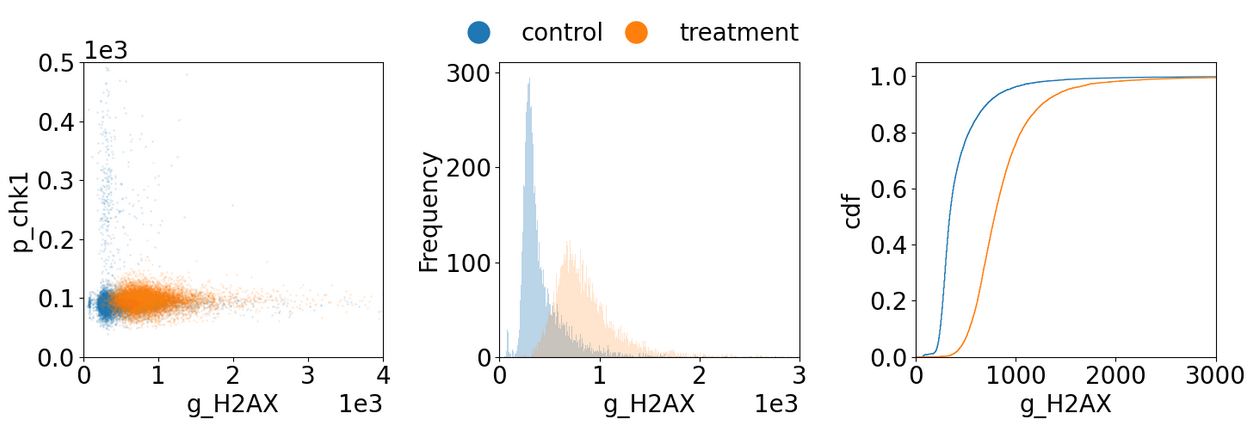
\includegraphics[clip, width=1\linewidth]{figures/ncs.png}\hspace*{\fill}}
    \caption{Automated immunofluorescence imaging against $\gamma$H2AX and phosphorylated Chk1 with a sample size of N=11000 for control and treatment each.}
    {\label{fig:ncs}}
\end{figure}

\paragraph*{} Using this tool, we pushed the limit of sample size for a damage response experiment based on immunofluorescence against $\gamma$H2AX and phosphorylated Chk1. We chemically induced damage, and imaged a total of 22000 cells, (11000 each for control and treated) with no human effort in imaging (Fig. \ref{fig:ncs}). This is far higher cell numbers than what is regularly done in microscopic investigations of DDR using everyday widefield microscopes. High Content microscopes can achieve such numbers, but we have now implemented this solution on a regular motorized widefield microscope, increasing the breadth of such investigations.

\begin{figure}[H]
    {\hfill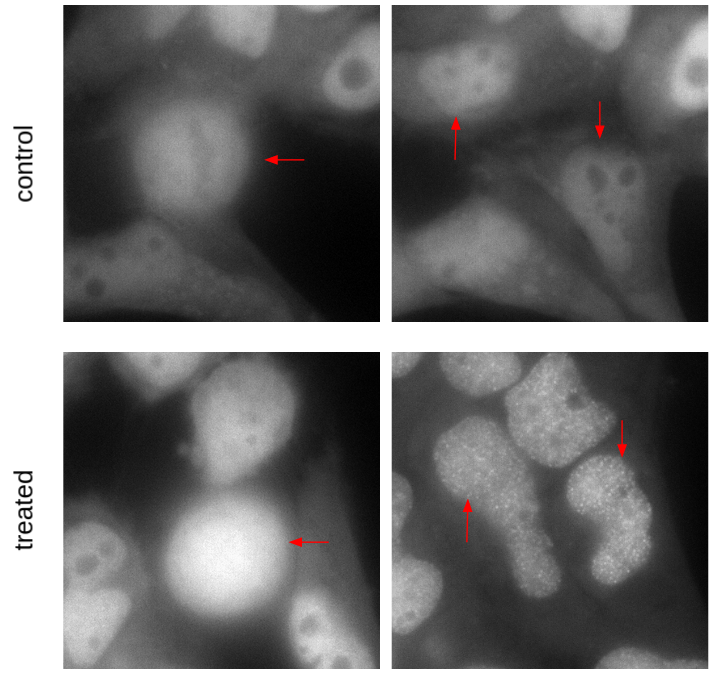
\includegraphics[clip, width=0.8\linewidth]{figures/g1.png}\hspace*{\fill}}
    \caption{G1 cells show punctated PCNA upon 4NQO damage. We followed mitotic cells (left) over time, until they divided into G1 cells. Treated G1 cells show punctated PCNA. The arrows are marking parent (left) and daughter cells (right)}
    {\label{fig:g1}}
\end{figure}

\paragraph*{} We further developed this tool to image live cells over high cell numbers to identify small subpopulations of interest. We imaged a large volume of HeLa cells expressing PCNA-chromobody, and induced damage with 4NQO. We observed that PCNA is punctated in non-S phase cells, indicating foci of repair. Furthermore, we also observed that damage foci are transferred to daughter G1 cells from a dividing mitotic cell (Fig. \ref{fig:g1}). This required us to acquire data over hundreds of cells in an asynchronous population. Potentially such studies can be done by chemically arresting cells in specific stages of the cell cycle and then releasing them. But such arrests themselves can alter measured responses, and there is value in performing studies in unperturbed asynchronous cultures.

\paragraph*{} In summary, we assembled a microscope acquisition software from scratch for hands-free high throughput data acqusition. We applied it to DDR and saw that we can push the sample size of traditional immunofluorescene experiments to N greater than 10,000 with no effort from the user. We increased throughput for live-cell imaging, and saw that PCNA foci form in bona fide G1 cells created right after a mitosis event.
